\documentclass{article}
\usepackage{tikz, comment}
\usepackage{pifont}
\usepackage{fontspec}
\usetikzlibrary{arrows, decorations.markings, decorations.pathreplacing}
\begin{comment}
:Title: Not defined yet
:Tags: foci of a hyperbola;focus of a parabola;directrices of a hyperbola;focal radius ;hyperbola
:Prob: 0.5124;0.4485;0.4368;0.4293;0.4279
:Slug: No name yet

Description Here.........
\end{comment}
\begin{document}\centering

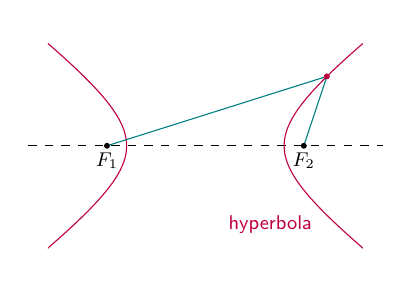
\begin{tikzpicture}[>=latex,xscale=.5*0.5, yscale=.5*0.5][font=\sf\small]

\draw[dashed] (-9, 0) -- (9, 0);

\clip[] (-8,-6) rectangle (8,6);

\draw[purple, samples=100, smooth, domain=-2:2, variable=\t]
plot ({4*cosh(\t)}, {3*sinh(\t)}) ;

\draw[purple, samples=100, smooth, domain=-3:3, variable=\t]
plot ({-4*cosh(\t)}, {3*sinh(\t)}) ;

\draw[teal] (-5,0) -- ({4*cosh(1)}, {3*sinh(1)}) -- (5, 0);

\draw[fill, xscale=1/0.5, yscale=1/0.5] (-5*0.5, 0) circle(0.06) node[below, scale=0.8]{$F_1$};
\draw[fill, xscale=1/0.5, yscale=1/0.5] ( 5*0.5, 0) circle(0.06) node[below, scale=0.8]{$F_2$};

\draw[purple, fill, xscale=1/0.5, yscale=1/0.5] ({4*cosh(1)*0.5}, {3*sinh(1)*0.5}) circle(0.06);

\node[purple, scale=0.8] at (3.3, -4) {$\hbox{hyperbola}$};

\end{tikzpicture}
\end{document}